\documentclass[a4paper]{article}

\usepackage{color}
\usepackage{url}
\usepackage[T2A]{fontenc}
\usepackage[utf8]{inputenc}
\usepackage{graphicx}

\usepackage[english, serbian]{babel}

\usepackage[unicode]{hyperref}
\hypersetup{colorlinks,citecolor=green,filecolor=green,linkcolor=blue,urlcolor=blue}
\newtheorem{primer}{Primer}[section]

\begin{document}

\title{Алфред Ахо\\ \small{Семинарски рад у оквиру курса\\Техничко и научно писање\\Математички факултет}}

\author{Богдан Марковић (bogdanis799@gmail.com),\\Јелена Максимовић (maksimovicj999@gmail.com),\\ Марија Чулић (marija.culic6@gmail.com)\\ Ђорђе Брадоњић (djordjebradonjic99@gmail.com)\\}
\date{4. новембар 2019.}
\maketitle

\abstract

У овом тексту укратко је приказана каријера Алфреда Ахоа. Описан је његов истраживачки рад у области информатике, указано је на најбитније радове и пројекте, посебно у оквиру алгоритама и интерпретираних програмских језика. Представљене су Ахоове значајне награде и вредност рада на Универзитету Колумбија. На тај начин показујемо значај овог канадског научника за развитак информатике, плана и програма учења информатичке науке на универзитетима.

\tableofcontents

\newpage

\section{Увод}
\label{sec:uvod}
\textbf{Алфред Ваино Ахо} (9. август 1941. године) канадски је информатичар најпознатији по свом раду на програмским језицима, преводиоцима и сродним алгоритмима и уџбеницима о уметности и науци рачунарског програмирања. Ахо је професор емеритус Катедре за рачунарске науке Универзитета Колумбија.

\begin{figure}[h!]
\begin{center}
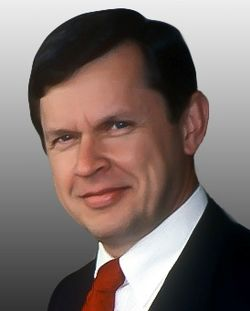
\includegraphics[scale=1.75]{AlfredAhoPortrait.jpg}
\end{center}
\caption{Алфред Ахо}
\end{figure}


\section{Каријера}
\label{sec:naslov1}
\subsection{Школовање}
\label{subsec:podnaslov1}

Алфред Ахо дипломирао је инжењерску физику на Универзитету у Торонту, а  докторирао у области електротехнике/рачунарских наука на Универзитету Принстон. Ментор му је био професор Џон Хопкрофт \cite{johnh}.

\subsection{Рад у Беловим лабораторијама}
\label{subsec:podnaslov2}
Након што је дипломирао на Принстону, Ахо је почео са радом на истраживањима у Беловим лабораторијама. На њима је радио најпре од 1967. до 1991. године, па од 1997. до 2002. као потпредседник Истраживачког центра за рачунарство (eng. \emph{Computing Sciences Research Center}). Осмислио је ефикасне алгоритме регуларног изражавања и слагања узорака и имплементирао их у првим верзијама Уникс алата \verb|egrep| и \verb|fgrep|. Алгоритам \verb|fgrep| постао је познат под називом Ахо-Корасикин алгоритам. Користи га неколико библиографских система за претрагу, укључујући онај који је развила Маргарет Ј. Корасик, и друге апликације за претраживање стрингова. 

У Беловим лабораторијама, Ахо је блиско сарађивао са Стивом Џонсоном и Џефријем Улманом на развоју ефикасних алгоритама за анализу и превођење програмских језика. Стив Џонсон је користио LALR алгоритме за парсирање како би створио генератор парсера \emph{yacc}, а Мајкл Е. Леск и Ерик Шмит користили су Ахоове алгоритме за усклађивање регуларних израза како би створили генератор лексера \emph{lex}. Алати \emph{lex} и \emph{yacc} и њихови деривати коришћени су за развој фронт-енд компоненти многих данашњих преводилаца програмских језика. 

\subsection{Рад на компајлерима}
\label{subsec:podnaslov3}
Ахо и Улман написали су низ уџбеника о техникама компајловања који су кодификовали теорију релевантну за дизајн компајлера. Њихов уџбеник из 1977. године Принципи дизајна компајлера (eng. \emph{Principles of Compiler Design}) имао је зеленог змаја на предњој корици и постао је познат као „Књига о зеленом змају". Године 1986. Аху и Улману придружио се Рави Сети како би створили ново издање, „Књигу о црвеном змају“ (која је накратко приказана у филму „Хакери“ из 1995. године), а 2007. и Моника Лам да би створили „Књигу о љубичастом змају". Књиге о змају најшире су коришћени уџбеници о компајлерима на свету. 

\subsection{Алгоритми}
\label{subsec:podnaslov4}
Године 1974. Ахо, Џон Хопкрофт и Улман написали су Дизајн и анализу рачунарских алгоритама (eng. \emph{Design and Analysis of Computer Algorithms}), кодификујући нека од својих ранијих истраживања алгоритама. Ова књига постала је једна од најтраженијих у рачунарској науци током неколико деценија и подстицала је стварање алгоритама и структура података као централног курса у наставном плану и програму информатике.


\subsection{Програмски језици}
\label{subsec:podnaslov5}
Алфред Ахо развио је програмски језик AWK заједно са Питером Ј. Вајнбергером и Брајаном Кернигеном ("А" означава "Аhо", "W" Weinberger, a "K" Kernighan). AWK се може посматрати као претходник Перла (слободни, независни од платформе и интерпретирани програмски језик којег је развио Aмериканац Лери Вол 1987. године).То је интерпретирани програмски језик дизајниран за обраду текста и најчешће коришћен као алатка за извожење података и за извештаје.Један је од стандардних алата на Уникс-базираним оперативним системима.

\subsection{Ахо као професор}
\label{subsec:podnaslov6}
Алфред Ахо има титулу професор емеритус на Универзитету Колумбија, што представља редовног професора у пензији који се посебно истакао својим научним радом. Катедри за рачунарске науке придружио се 1995. године и председавао Катедром од 1995. до 1997. године, па поново на пролеће 2003. године. За свој рад награђен је 2003. од стране Друштва дипломаца Колумбије. 

\subsection{Признања}
\label{subsec:podnaslov7}
Алфред Ахо примио је многа престижна признања, укључујући IEEE-ову Медаљу Џона фон Нојмана (eng. \emph {John von Neumann Medal}) и чланство у Националној инжењерској академији (eng. \emph {National Academy of Engineering}). Изабран је за члана Америчке академије наука и уметности (eng. \emph {American Academy of Arts and Sciences}) 2003. године. Има почасне докторате са Универзитета у Ватерлоу, са Универзитета у Хелсинкију, са Универзитета у Торонту, и члан је Америчког удружења за унапређење науке (eng. \emph{American Association for the Advancement of Science}) , ACM-а (Association for Computing Machinery), Белових лабораторија и IEEE-а (eng. \emph {Institute of Electrical and Electronics Engineers}). 


\begin{table}[h!]
\begin{center}
\caption{Ахоова признања и награде}
\begin{tabular}{|l|l|} \hline
награда& година\\ \hline
Bell Labs Fellow &1984\\ \hline
FAAAS &1986\\ \hline
IEEE Fellow &1988\\ \hline
FACM &1996\\ \hline
IEEE John von Neumann Medal &2003\\ \hline
NAE Member &\\ \hline

\end{tabular}
\label{tab:tabela1}
\end{center}
\end{table}

\section{Књиге}

\label{sec:knjige}

\begin{itemize}
    \item Edward K. Blum and Alfred V. Aho (eds.)
    Computer Science: The Hardware, Software and Heart of It
    Springer, 2011 
    
    \item Alfred V. Aho, Monica S. Lam, Ravi Sethi, and Jeffrey D. Ullman
    Compilers: Principles, Techniques, & Tools, Second Edition
    Boston: Addison-Wesley, 2007 
    
    \item Alfred V. Aho and Jeffrey D. Ullman
    Foundations of Computer Science with C
    New York: W. H. Freeman/Computer Science Press, 1995
    
    \item Alfred V. Aho and Jeffrey D. Ullman
    Foundations of Computer Science
    New York: W. H. Freeman/Computer Science Press, 1992 
    
    \item Alfred V. Aho, Brian W. Kernighan, and Peter J. Weinberger
    The AWK Programming Language
    Reading, Massachusetts: Addison-Wesley, 1988 
    
    \item Alfred V. Aho, Ravi Sethi, and Jeffrey D. Ullman
    Compilers: Principles, Techniques, and Tools
    Reading, Massachusetts: Addison-Wesley, 1986

    \item Alfred V. Aho, John E. Hopcroft, and Jeffrey D. Ullman
    Data Structures and Algorithms
    Reading, Massachusetts: Addison-Wesley, 1983

    \item Alfred V. Aho and Jeffrey D. Ullman
    Principles of Compiler Design
    Reading, Massachusetts: Addison-Wesley, 1977
    
    \item Alfred V. Aho, John E. Hopcroft, and Jeffrey D. Ullman
    The Design and Analysis of Computer Algorithms
    Reading, Massachusetts: Addison-Wesley, 1974

    \item Alfred V. Aho and Jeffrey D. Ullman
    The Theory of Parsing, Translation, and Compiling, Volume 2: Compiling
    Englewood Cliffs, N.J.: Prentice-Hall, 1973

    \item Alfred V. Aho (ed.)
    Currents in the Theory of Computing
    Englewood Cliffs, N.J.: Prentice-Hall, 1973

    \item Alfred V. Aho and Jeffrey D. Ullman
    The Theory of Parsing, Translation, and Compiling, Volume 1: Parsing
    Englewood Cliffs, N.J.: Prentice-Hall, 1972



    
\end{itemize}
\section{Закључак}
\label{sec:zakljucak}
Значајна признања, чланство на престижним универзитетима и академијама, као и почасне титуле и звања, сведоче да је Алфред Ахо информатичар великог формата. Ахоов рад у Беловим лабораторијама, интересовање за програмске језике и алгоритме, али и коауторство иновативних уџбеника о техникама компајлера, драгоцено су полазиште за будућа изучавања информатичке науке.
\addcontentsline{toc}{section}{Литература}
\appendix
\bibliography{AlfredAho}
\bibliographystyle{plainnat}


\end{document}
                  
